\documentclass[12pt,twoside]{article}
\linespread{1.5} 
\usepackage{textgreek}
\usepackage [english, greek] {babel}
\usepackage[numbers]{natbib}
\usepackage{url}
\usepackage[utf8x]{inputenc}
\usepackage{amsmath}
\usepackage{graphicx}
\graphicspath{{images/}}
\usepackage{rotating}
\usepackage{fancyhdr}
\usepackage{lettrine}
\usepackage{type1cm}
\usepackage{vmargin}
\setmarginsrb{3 cm}{1.5 cm}{3 cm}{2.5 cm}{1 cm}{1.5 cm}{1 cm}{1.5 cm}
\usepackage{bm}
\usepackage{csquotes}
\renewcommand*\descriptionlabel[1]{\hspace\leftmargin$#1$}
\usepackage{enumitem} 
\usepackage{commath}
\usepackage{amsfonts}
\usepackage{listings}
\usepackage{breakcites}
\usepackage{url}
\usepackage{footnote}
%\usepackage{slashbox}
\usepackage[nottoc]{tocbibind}
\usepackage{subfigure}
\usepackage{algorithmic, algorithm, listings}
\usepackage[caption=false, font=footnotesize]{subfig}
\usepackage[export]{adjustbox}
\renewcommand{\algorithmicrequire}{\textbf{Input:}}
\renewcommand{\algorithmicensure}{\textbf{Output:}}
\setcitestyle{square}
\newcommand{\en}{\selectlanguage{english}}
\newcommand{\gr}{\selectlanguage{greek}}
\newcommand\blfootnote[1]{%
  \begingroup
  \renewcommand\thefootnote{}\footnote{#1}%
  \addtocounter{footnote}{-1}%
  \endgroup
}
\gr
\title{\gr Αξιοποίηση της ανάλυσης χρονοσειρών στο \en Twitter \gr για τον  υπολογισμό της απόδοσης μιας καμπάνιας}                                
\makeatletter
\let\thetitle\@title
\let\theauthor\@author
\let\thedate\@date
\makeatother

\pagestyle{fancy}
\fancyhf{}
\fancyhead[LE,RO]{\itshape\nouppercase{\rightmark}}
\cfoot{\thepage}

\begin{document}
\raggedbottom
\makeatletter
\def\@seccntformat#1{%
  \expandafter\ifx\csname c@#1\endcsname\c@section\else
  \csname the#1\endcsname\quad
  \fi}
\makeatother
%%%%%%%%%%%%%%%%%%%%%%%%%%%%%%%%%%%%%%%%%%%%%%%%%%%%%%%%%%%%%%%%%%%%%%%%%%%%%%%%%%%%%%%%%

\begin{titlepage}
\en
    \centering

    
\includegraphics[scale = 0.75]{logo.png}\\[0.0 cm]  % University Logo

    \textsc{ \gr \Huge Πολυτεχνική Σχολή \\ Τμημα μηχανικων η/υ και πληροφορικης}\\[0.5 cm]  % University Name

    \rule{\linewidth}{0.2 mm} \\[0.4 cm]
    { \Large \bfseries \thetitle}\\
    \rule{\linewidth}{0.2 mm} \\[0.4 cm]

    \gr \textbf{\Large{ΔΙΠΛΩΜΑΤΙΚΗ ΕΡΓΑΣΙΑ}\\}
    \large {του Γεράσιμου Λ. Ρόμπολα}\\[1.0cm]

    
    \begin{minipage}{0.4\textwidth}
        \begin{flushleft} \normalsize
            \textbf{\emph{\gr Επιβλέπων:}\\}
\vspace{-0.2cm}
            \gr Χρήστος Μακρής\\
\vspace{-0.2cm}
            \gr Αναπληρωτής Καθηγητής\\
\vspace{-0.2cm}
            \gr Τμήμα Μηχανικών Η/Υ και \\
\vspace{-0.2cm} 
           Πληροφορικής\\
\vspace{-0.2cm}
	    \gr Πανεπιστήμιο Πατρών\\
	    \null
            \end{flushleft}
            \end{minipage}~
            \begin{minipage}{0.4\textwidth}
            
            \begin{flushright} \normalsize
            \textbf{\emph{\gr Συνεπιβλέπουσα:} \\}
\vspace{-0.2cm}
            \gr Ελεάννα Καφέζα\\
\vspace{-0.2cm}
            \gr Επίκουρη Καθηγήτρια\\
\vspace{-0.2cm}
            \gr Τμήμα Μάρκετινγκ και \\
\vspace{-0.2cm}
            Επικοινωνίας\\
\vspace{-0.2cm}
	    \gr Οικονομικό Πανεπιστήμιο\\ 
\vspace{-0.2cm}
	    Αθηνών
        \end{flushright}
        
    \end{minipage}\\[0.5 cm]
    
    \gr \small {\textbf{Πάτρα, Σεπτέμβριος 2017 }}
        
\end{titlepage}

\pagenumbering{roman}
\newpage
\vspace*{\fill}
\hspace{-7.5mm}
\textbf{\en Copyright © \gr Γεράσιμος Λ. Ρόμπολας, 2017\\
Με επιφύλαξη παντός δικαιώματος. \en All rights reserved.\gr\\}
\hspace{-7.5mm}\\
\textbf{Απαγορεύεται}  η  αντιγραφή, η αποθήκευση  και η διανομή  της  παρούσας  εργασίας,  εξ’ ολοκλήρου ή τμήματος αυτής, για εμπορικό σκοπό.
Επιτρέπεται η ανατύπωση, η αποθήκευση και η διανομή  για  σκοπό  μη-κερδοσκοπικό,  εκπαίδευσης  ή  ερευνητικής  φύσης,  υπό  την 
προϋπόθεση  να  αναφέρεται  η  πηγή  προέλευσης  και  να διατηρείται το  παρόν  μήνυμα. 
Ερωτήματα  που  αφορούν  τη  χρήση  της  εργασίας  για  κερδοσκοπικό  σκοπό  πρέπει  να 
απευθύνονται προς τον συγγραφέα.\\
\hspace{-7.5mm}\\
Οι  απόψεις  και  τα  συμπεράσματα  που  περιέχονται  σε  αυτό  το  έγγραφο  εκφράζουν  τον 
συγγραφέα  και  δεν  πρέπει  να  ερμηνευθεί  ότι  αντιπροσωπεύουν  τις  επίσημες  θέσεις  του 
Πανεπιστημίου Πατρών.
\blfootnote{\gr Το παρόν πρότυπο \LaTeX \hspace{0mm} έχει δημιουργηθεί από τον Γεράσιμο Ρόμπολα.}
\thispagestyle{empty}
\newpage
\setcounter{page}{1}

%ΠΕΡΙΛΗΨΗ
\thispagestyle{plain}
\paragraph{\Large{\gr Περίληψη}}
\
\\
\vspace{-0.7cm}
\gr
\lettrine[loversize=0.03]{\en E}{\gr νώ} οι επιχειρήσεις διαθέτουν μία πληθώρα μετρικών για τον υπολογισμό της απόδοσης των επιχειρηματικών διαδικασιών τους, πρόσφατα έχει εμφανιστεί η ανάγκη αξιολόγησής τους με βάση το βαθμό επιρροής των καταναλωτών. Στη θεωρία του σύγχρονου μάρκετινγκ τα κοινωνικά δίκτυα αποτελούν ένα από τα σημαντικότερα μέσα προώθησης προϊόντων και υπηρεσιών. Συνεπώς, η εργασία αυτή επικεντρώνεται στην αξιολόγηση της απόδοσης μιας επιχειρηματικής διαδικασίας με βάση την επίδρασή της σε ένα δημοφιλές και δυναμικό κοινωνικό δίκτυο, όπως το \en Twitter\gr.
\vspace{-6mm}
\paragraph{}Συγκεκριμένα, στην εργασία αυτή προτείνεται ένας νέος τρόπος υπολογισμού των σχέσεων \textquote{\en follow} μεταξύ των χρηστών, στο \en Twitter\gr. Η νέα αυτή προσέγγιση βασίζεται στις αντιδράσεις των χρηστών ως προς τις δραστηριότητες μίας καμπάνιας μάρκετινγκ, αξιοποιώντας τη συστημική ανάλυση χρονοσειρών και συναισθήματος για τον καθορισμό και τον υπολογισμό της απόδοσής της. Στη συνέχεια, ο κοινωνικός γράφος του δικτύου \en Twitter \gr ανακατασκευάζεται, αξιοποιώντας τη συμπεριφορά των χρηστών ως προς τις δραστηριότητες μάρκετινγκ της επιχείρησης. Τέλος, για τον προσδιορισμό και την εξαγωγή κοινοτήτων στενά συνδεδεμένων χρηστών χρησιμοποιείται αντίστοιχα ένας αλγόριθμος ανίχνευσης κοινοτήτων και επομένως καθορίζονται οι απαραίτητες μετρικές για  τον υπολογισμό της απόδοσης της καμπάνιας μάρκετινγκ.
\vspace{-6mm}
\paragraph{}Για την αξιολόγηση της προτεινόμενης μεθοδολογίας, γίνεται η αξιοποίηση ενός συνόλου δεδομένων βασισμένο σε ένα πολιτικό πρόσωπο, με σκοπό την ανακατασκευή της μάρκετινγκ καμπάνιας του ως ένα σύνολο δραστηριοτήτων, χρησιμοποιώντας τον αλγόριθμος λανθάνουσας κατανομής του \en Dirichlet (LDA)\gr. Τα αποτελέσματα της νέας προσέγγισης δείχνουν ότι η συστημική ανάλυση κοινωνικών δικτύων μπορεί να αποτελέσει μία έγκαιρη και αξιόπιστη μετρική για την αξιολόγηση της απόδοσης μιας επιχειρηματικής διαδικασίας μάρκετινγκ.

\paragraph{\large{\gr Λέξεις Κλειδιά:}}
 ανάλυση χρονοσειρών, ανίχνευση κοινοτήτων, επιχειρηματική διαδικασία καμπάνιας μάρκετινγκ, συστημική ανάλυση δεδομένων


\newpage
\thispagestyle{empty}
\null


%ABSTRACT
\newpage
\thispagestyle{plain}
\paragraph{\Large{\en Abstract}}
\
\\
\vspace{-0.7cm}
\en
\lettrine{W}{hile} businesses have a plethora of metrics to measure the performance of their business processes, recently has emerged the requirement for their evaluation based on the degree of consumer influence. In the theory of modern marketing, social networks are one of the most important means of promoting products and services. Consequently, this work focuses on evaluating the performance of a business process based on its impact on a popular and dynamic social network, such as Twitter.

\vspace{-6mm}
\paragraph{}
Specifically, this work proposes a new way of calculating the "follow" relationships between users, on Twitter. This new approach is based on users' reactions to the marketing campaign activities, exploiting time series and sentiment analysis for defining and measuring their performance. Then, Twitter's social graph is being reconstructed, exploiting users' behavior towards business marketing activities. Finally, in order to identify and export communities of densely connected users, a community detection algorithm is used, and therefore the necessary metrics are being defined to measure the performance of the marketing campaign.

\vspace{-6mm}
\paragraph{}
In order to evaluate the proposed methodology, a dataset based on a specific politician is being used to rebuild its marketing campaign as a set of activities using the Latent Dirichlet Allocation algorithm (LDA). The results of the new approach show that social network analytics can be a valid and reliable metric for assessing the performance of a marketing campaign business process.

\paragraph{\large{\en Keywords:}}
community detection,  data analytics, marketing campaign business process, time series analysis



\newpage\null
\thispagestyle{plain}
\vspace*{\fill}
\begin{center}
\begin{minipage}{.6\textwidth}
\centering \textbf{\en\textit{ “The saddest aspect of life right now is that science gathers knowledge faster than society gathers wisdom.”}
\rightline{{\rm ---  Isaac Asimov}}}%\gr Σκοπίμως κενή σελίδα}
\end{minipage}
\end{center}
\vfill


%ΕΥΧΑΡΙΣΤΙΕΣ
\newpage
\thispagestyle{plain}
\paragraph{\Large{\gr Ευχαριστίες}}
\paragraph{}
\gr Θα ήθελα να ευχαριστήσω τον καθηγητή κ. Χρήστο Μακρή για την επίβλεψη αλλά και για τη συμβολή του στην εκπόνηση αυτής της διπλωματικής εργασίας. Επίσης ευχαριστώ θερμά την καθηγήτρια κα. Ελεάννα Καφέζα για την καθοδήγησή της και για την εξαιρετική συνεργασία που είχαμε. 
\paragraph{}
Τέλος θα ήθελα να ευχαριστήσω τους γονείς μου για τη υποστήριξη και την ηθική συμπαράσταση που μου προσέφεραν όλα αυτά τα χρόνια.

\hspace{8cm} \textbf{\textit{Πάτρα, 1 Σεπτεμβρίου 2017}}


\newpage
\thispagestyle{empty}
\null

\gr
\newpage
\thispagestyle{plain}
\tableofcontents

\newpage
\thispagestyle{empty}
\null

\gr
\newpage
\thispagestyle{plain}
\listoffigures

\newpage
\thispagestyle{empty}
\null

\newpage
\thispagestyle{plain}
\listoftables

\newpage\null
\thispagestyle{empty}

\pagebreak
\pagenumbering{arabic}
%%%%%%%%%%%%%%%%%%%%%%%%%%%%%%%%%%%%%%%%%%%%%%%%%%%%%%%%%%%%%%%%%%%%%%%%%%%%%%%%%%%%%%%%%




%ΕΙΣΑΓΩΓΗ
\newpage
\thispagestyle{plain}
\null
\vspace{2cm}
\hspace{-6.5mm}{\textbf{\Huge
 \gr Κεφάλαιο 1}}
\vspace{-4mm}
\section{\gr Εισαγωγή}
\gr
\lettrine[loversize=0.03]{\en H}{\gr }
 ραγδαία ανάπτυξη των τηλεπικοινωνιών και της μεταφοράς δεδομένων στα τέλη του 20ου αιώνα, αποτέλεσε ακρογωνιαίο λίθο για την γέννηση του Διαδικτύου. Η αρχική μορφή του Διαδικτύου περιοριζόταν στην εξυπηρέτηση συστημάτων που βασίζονταν αποκλειστικά σε κείμενο και στις υπηρεσίες ηλεκτρονικού ταχυδρομείου. Ώσπου το 1990,  ο Βρετανός \en Sir Tim Berners-Lee \gr μαζί με τον Βέλγο \en Robet Cailliau \gr πρότειναν ένα σύστημα υπερκειμένου \cite{connolly2014fundamentals}. Οι δυνατότητες του συστήματος υπερκειμένου κατέστησαν εφικτή τη διασύνδεση ιεραρχημένων στοιχείων, εξασφαλίζοντας τη χρήση εικόνας και ήχου. Το σύστημα αυτό χρησιμοποιείται ως σήμερα και είναι γνωστό ως ο Παγκόσμιος Ιστός. 

Το πρώτο στάδιο της εξέλιξης του Παγκόσμιου Ιστού ονομάστηκε ως \en Web 1.0. \gr Οι χρήστες δρούσαν παθητικά, όντας απλοί καταναλωτές της πληροφορίας, καθώς ο Παγκόσμιος Ιστός ήταν κατακλυσμένος από ένα σύνολο στατικών ιστοσελίδων.  Σταδιακά, με την εμφάνιση νέων τεχνολογικών μέσων και εργαλείων εξελίχτηκε στο δεύ-τερο στάδιο, που ονομάστηκε αντίστοιχα ως \en Web 2.0. \gr Αυτή η γενιά 
χαρακτηρίστηκε από την δυναμικότητα που προσέφερε, δίνοντας τη δυνατότητα άμεσης αλληλεπίδρασης μεταξύ των χρηστών. Χαρακτηριστικό στοιχείο της γενιάς αυτής αποτελεί η εφεύρεση των κοινωνικών δικτύων, μέσω των οποίων οι χρήστες μπορούσαν να εκφραστούν και να επικοινωνούν όπως ποτέ άλλοτε. Η γενιά του \en Web 2.0 \gr είναι εκείνη που επικρατεί ως και σήμερα στον Παγκόσμιο Ιστό. Το επόμενο στάδιο στης εξέλιξής του θεωρείται ότι θα είναι αντίστοιχα το \en Web 3.0, \gr διαδεδομένο και ως σημασιολογικός ιστός, \gr το οποίο θα προσθέτει σημασιολογικά στοιχεία στη δομή των ιστοσελίδων.  

Η δημιουργία των κοινωνικών δικτύων στον Παγκόσμιο Ιστό, οδήγησε τους χρήστες στην άμεση μεταξύ τους επαφή, να μοιράζονται και να ανταλλάσσουν περιεχόμενο σε ένα ελεύθερο περιβάλλον. Η δυνατότητα αυτή των κοινωνικών δικτύων έλκυσε εκατομμύρια ανθρώπους, με αποτέλεσμα ο όγκος του διαμοιραζόμενου περιεχομένου να αυξηθεί αλματωδώς. 

Παράλληλα με την καταιγιστική ροή δεδομένων, οι χρήστες απαίτησαν από αυτά πιο εξειδικευμένες πληροφορίες. Χαρακτηριστικό παράδειγμα αποτελεί ο τομέας ανάλυσης και διαχείρισης της αγοράς, όπου η ανάλυση δεδομένων είναι ιδιαίτερα σημαντική για την πορεία των επιχειρήσεων. Συγκεκριμένα, οι επιχειρήσεις ενδιαφέρονται για τη στοχοποίηση των διαφημιστικών τους εκστρατειών σε υψηλά διασυνδεδεμένα σύνολα χρηστών, τον προσδιορισμό των προφίλ και των απαιτήσεων των πελατών, την ανάλυση και τη διαχείριση των κινδύνων, καθώς και την πρόβλεψη των αποθεμάτων τους με βάσει τις πωλήσεις. Περαιτέρω τομείς αφορούν τον εντοπισμό και τη διαχείριση του οικονομικού εγκλήματος, την ανακάλυψη βιολογικής γνώσης αλλά και την πρόβλεψη γεγονότων.

Για την ικανοποίηση αυτών των αναγκών χρησιμοποιούνται ως και σήμερα τεχνικές εξόρυξης δεδομένων και αλγόριθμοι μάθησης, μέσω των οποίων είναι εφικτό να εξαχθεί ή να παραχθεί λειτουργική γνώση που βρίσκεται κρυμμένη μέσα στα δεδομένα. 




%ΘΕΩΡΙΑ ΓΡΑΦΩΝ
\newpage
\thispagestyle{plain}
\null
\vspace{2cm}
\hspace{-6.5mm}{\textbf{\Huge
 \gr Κεφάλαιο 2}}
\vspace{-4mm}
\section{\gr Θεωρία Γράφων}
\gr
\lettrine[loversize=0.03]{\en T}{\gr α}
τελευταία χρόνια υπάρχει ένα διαρκώς αυξανόμενο ενδιαφέρον για τη μελέτη της δομής της σύγχρονης κοινωνίας ως απόρροια της ταχείας ανάπτυξης του Διαδικτύου και του Παγκόσμιου Ιστού. Η ευκολία με την οποία πραγματοποιείται τώρα η παγκόσμια επικοινωνία και η ταχύτητα με την οποία μεταδίδονται οι πληροφορίες και οι ειδήσεις είναι εκπληκτική. Οι άνθρωποι πλέον δίχως να περιορίζονται από γεωγραφικά όρια, έχουν τη δυνατότητα να έρχονται σε άμεση επαφή με άλλους πολιτισμούς, να ανταλλάσσουν και να μοιράζονται ιδέες και απόψεις. Το γεγονός αυτό έχει ως αποτέλεσμα τη δημιουργία ευρύτερων κοινωνικών ομάδων, οι οποίες με βάση τα κίνητρά τους και τη συμπεριφορά τους μπορούν να επέμβουν και να επηρεάσουν σημαντικά τη ζωή άλλων ανθρώπων. 

Με γνώμονα αυτές τις παγκόσμιες εξελίξεις, οι επιστημονικοί κλάδοι παρακινήθηκαν και συνεργάστηκαν για να κατανοήσουν τον τρόπο λειτουργίας της σύγχρονης κοινωνίας, αλλά και παρόμοιων υψηλά διασυνδεδεμένων δικτύων. Συγκεκριμένα, από την επιστήμη των υπολογιστών και των μαθηματικών προήλθε ένα συλλογιστικό πλαίσιο ερμηνείας της αύξησης της πολυπλοκότητας των δικτύων. Από τις κοινωνικές επιστήμες εντοπίστηκαν χαρακτηριστικές δομές και αλληλεπιδράσεις που εμφανίζονται μέσα σε κοινωνικές ομάδες. Και από την επιστήμη των οικονομικών ερμηνεύθηκε η επιρροή της συμπεριφοράς των ανθρώπων από τα κίνητρα και τις προσδοκίες τους. Είναι φανερό ότι κάθε επιστημονικός κλάδος συνεισφέρει αποκλειστικά δικές του γνώσεις και τεχνικές. Ωστόσο η σύνθεση όλων των συσχετιζόμενων επιστημονικών κλάδων έχει οδηγήσει στη μελέτη ακόμα πιο σύνθετων δομών δικτύων, αξιοποιώντας ταυτόχρονα γνώσεις από όλους τους αντίστοιχους κλάδους. 

Η σύνθετη μορφή αυτή του κάθε δικτύου χαρακτηρίζεται από υψηλή πολυπλοκότητα και είναι γενικά δύσκολο να εξαχθεί μια πλήρης εικόνα για τη συνολική μορφή του. Για τη μελέτη της διάρθρωσής των δικτύων είναι απαραίτητη η κατανόηση βασικών εννοιών της θεωρίας γράφων, καθώς αποτελεί το βασικό μοντέλο περιγραφής των δικτύων.  



\subsection{\gr Βασικές έννοιες}
\paragraph{}\gr
Με σκοπό την περιγραφή και την κατανόηση των δομών των δικτύων, περιγράφονται αρχικά μερικοί από τους βασικούς ορισμούς και συμβολισμούς της θεωρίας γράφων. 

\subsubsection{\gr (Μη) Κατευθυνόμενοι γράφοι}
\paragraph{}\gr
Ένας κοινός ορισμός ενός γράφου είναι η απεικόνιση των σχέσεων μεταξύ ενός συνόλου αντικειμένων και συμβολίζεται συνήθως ως $G=\{V, E\}$. Ο γράφος $G$ αποτελείται από ένα σύνολο σημείων, $V$, που ονομάζονται κόμβοι, καθώς και από ένα σύνολο συνδέσεων μεταξύ των κόμβων, $E$, που ονομάζονται ακμές. Δύο κόμβοι ονομάζονται γειτονικοί μόνο εάν συνδέονται μέσω μίας ακμής. Στο Σχήμα \ref{gr} αναπαρίσταται ένας τυπικός τρόπος σχεδιασμού ενός γράφου, αναπαριστώντας τους κόμβους με κύκλους και τις ακμές μεταξύ 2 κόμβων με ευθύγραμμα τμήματα. Συγκεκριμένα, ο γράφος $G_1$ αποτελείται από τέσσερις κόμβους τους Α, Β, Γ και Δ , με τον κόμβο Β να συνδέεται με κάθε έναν από τους υπόλοιπους κόμβους μέσω ακμών, και από μία επιπλέον ακμή μεταξύ των κόμβων Α και Γ. 

Στο γράφο $G_1$ του Σχήματος \ref{gr}(α'), η σχέση μεταξύ δύο διασυνδεδεμένων κόμβων θεωρείται συμμετρική. Ωστόσο, σε πολλές περιπτώσεις υπάρχει η ανάγκη έκφρασης ασυμμετρικών σχέσεων. Για παράδειγμα ο κόμβος Α να δείχνει στον κόμβο Β, αλλά χωρίς να ισχύει το αντίστροφο. Για τον σκοπό αυτό, ορίζεται η έννοια του κατευθυνόμενου γράφου, ο οποίος αποτελείται από ένα σύνολο διασυνδεδεμένων κόμβων μέσω ενός συνόλου κατευθυνόμενων ακμών. Κάθε κατευθυνόμενη ακμή δείχνει από τον έναν κόμβο στον άλλον, δίνοντας σημασία στην κατεύθυνση που δείχνει.  Οι κατευθυνόμενοι γράφοι σχεδιάζονται συνήθως όπως στο γράφο $\hat{G_1}$ του Σχήματος \ref{gr}(β'), όπου η κάθε κατευθυνόμενη ακμή αναπαρίσταται με τη χρήση ενός βέλους. Όταν γίνεται αναφορά σε έναν γράφο που δεν είναι κατευθυνόμενος, ονομάζεται ως μη κατευθυνόμενος γράφος. 

Η τάξη ενός γράφου ορίζεται ως το συνολικό πλήθος των κόμβων του και συμβολίζεται ως $\abs{V}$. Αντίστοιχα ορίζεται το μέγεθος ενός γράφου, ως το συνολικό πλήθος των ακμών του και συμβολίζεται ως $\abs{E}$. Επίσης, κάθε κόμβος ενός γράφου χαρακτηρίζεται από το βαθμό του, ο οποίος ισούται με το σύνολο των ακμών που συνδέονται σε αυτόν. 

\begin{figure*}[!t]
\centering
\subfigure[Μη κατευθυνόμενος γράφος $G_1$]{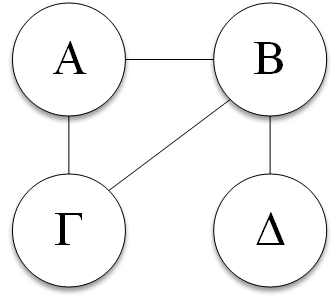
\includegraphics[width=0.36\textwidth]{graph1.png}}
	\hfil
	\subfigure[Κατευθυνόμενος γράφος $\hat{G_1}$]{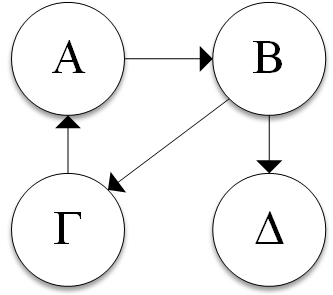
\includegraphics[width=0.36\textwidth]{graph2.png}}
 \caption{Δύο γράφοι αποτελούμενοι από 4 κόμβους και 4 ακμές}
 \label{gr}
\end{figure*}
\begin{figure*}[!t]
\centering
\subfigure[Μη κατευθυνόμενος γράφος $G_2$]{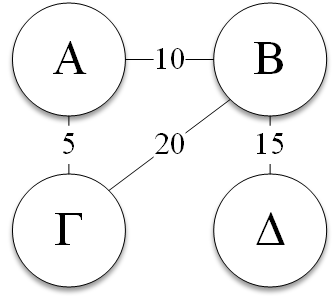
\includegraphics[width=0.36\textwidth]{weighted_graph1.png}}
	\hfil
	\subfigure[Κατευθυνόμενος γράφος $\hat{G_2}$]{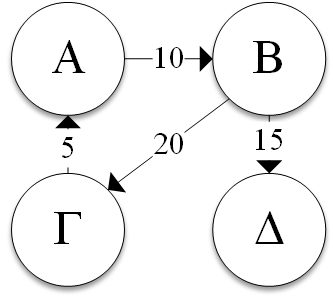
\includegraphics[width=0.36\textwidth]{weighted_graph2.png}}
 \caption{Δύο βεβαρημένοι γράφοι αποτελούμενοι από 4 κόμβους και 4 ακμές}
 \label{gr2}
\end{figure*}

Σε πολλές περιπτώσεις, κάθε ακμή ενός γράφου συσχετίζεται με μία αριθμητική τιμή, η οποία ονομάζεται βάρος. Συνήθως, τα βάρη των ακμών είναι μη αρνητικοί ακέραιοι αριθμοί. Ο γράφος που παρουσιάζει αυτή τη δομή ονομάζεται βεβαρημένος και μπορεί να είναι είτε κατευθυνόμενος, είτε μη κατευθυνόμενος, όπως οι γράφοι $G_2$ και $\hat{G_2}$ αντίστοιχα του Σχήματος \ref{gr2}. Το βάρος μίας ακμής ονομάζεται συχνά και ως κόστος της ακμής. Σε εφαρμογές, το βάρος μιας ακμής μπορεί να αναπαριστά ένα οποιαδήποτε μέτρο ανάμεσα στους δύο αντίστοιχους κόμβους που συνδέει. Για παράδειγμα, μπορεί να μετρά το μήκος ενός δρόμου, τη χωρητικότητα μιας γραμμής, την ενέργεια που απαιτείται για την μετακίνηση μεταξύ των κόμβων κτλ.



\subsection{\gr Αναπαράσταση γράφων}
\paragraph{}
Για την πρακτική αξιοποίηση των δομών των γράφων απαιτείται η αναπαράστασή τους σε μια κατάλληλη μορφή, ώστε να είναι επεξεργάσιμη και κατανοητή από τους ανθρώπους και τους υπολογιστές. Για το λόγο αυτό, στην επιστήμη των υπολογιστών αλλά και των μαθηματικών χρησιμοποιούνται αντίστοιχες δομές αναπαράστασης των δεδομένων ανάλογα με τα δομικά χαρακτηριστικά του γράφου. Ως επί το πλείστον, οι δομές αναπαράστασης γράφων που χρησιμοποιούνται είναι τα μητρώα (\en Adjacency matrices\gr) καθώς και οι λίστες γειτνίασης (\en Adjacency lists\gr). Κάθε δομή προσφέρει τα δικά της πλεονεκτήματα και μειονεκτήματα ανάλογα με το είδος της απαιτούμενης επεξεργασίας του γράφου. Για την περιγραφή των παραπάνω δομών, ορίζουμε ένα γράφο $G=(V,E)$, όπου $V$ είναι το σύνολο των κόμβων και $E$ είναι το σύνολο των ακμών αντίστοιχα. 


\subsubsection{\gr Μητρώο γειτνίασης}
\gr
\paragraph{}
Το μητρώο γειτνίασης χρησιμοποιείται για την αναπαράσταση των κόμβων ενός γράφου, καθώς και για τον τρόπο σύνδεσής τους με τους υπόλοιπους κόμβους. Για έναν πεπερασμένο γράφο $G=(V,E)$, το μητρώο γειτνίασης ορίζεται ως ένας πίνακας διαστάσεων $\abs{V}\times\abs{V}$, του οποίου τα στοιχεία $e_{i,j}$ ορίζονται ως εξής:

\en
\[
    e_{i,j}=\left\{
                \begin{array}{ll}
                  1, \; \alpha v \;  \exists \; \alpha\kappa\mu\acute{\eta}  \;  \mu\epsilon\tau\alpha\xi\acute{\upsilon} \; \tau\omega v \; \kappa \acute{o} \mu\beta\omega v \;  V_i \; \kappa\alpha\iota \;  V_j\\
                  0, \; \alpha\lambda\lambda \iota\acute{\omega}s
                \end{array}
              \right.
  \]

\gr
\paragraph{}
 Στην περίπτωση βεβαρημένου γράφου, ο παραπάνω ορισμός των στοιχείων του μητρώου γειτνίασης διαφοροποιείται. Συγκεκριμένα όταν υπάρχει ακμή μεταξύ δύο κόμβων, το στοιχείο του μητρώου $e_{i,j}$ ισούται με το βάρος της αντίστοιχης ακμής μεταξύ των κόμβων $V_i$ και $V_j$. Στην ειδική περίπτωση που ο γράφος είναι μη κατευθυνόμενος, το μητρώο γειτνίασης που προκύπτει παρουσιάζει συμμετρική μορφή. Για παράδειγμα, στα Σχήματα \ref{mat1} και \ref{mat2} παρουσιάζονται τα μητρώα γειτνίασης των γραφών που μελετήθηκαν ως τώρα, των Σχημάτων \ref{gr} και \ref{gr2} αντίστοιχα. 

\gr
\begin{figure*}[h]
\centering
\subfigure[Μη κατευθυνόμενου γράφου $G_1$]{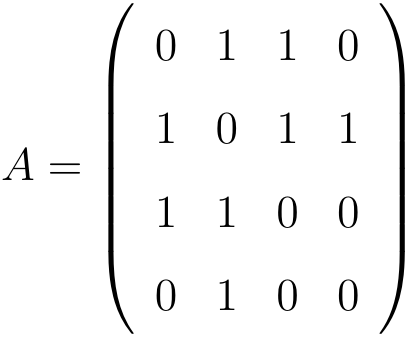
\includegraphics[width=0.25\textwidth]{adj_matrix1.png}}
	\hfil
	\subfigure[Κατευθυνόμενου γράφου $\hat{G_1}$]{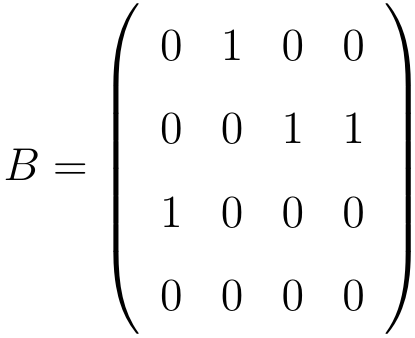
\includegraphics[width=0.25\textwidth]{adj_matrix2.png}}
\caption{Μητρώα γειτνίασης γράφων χωρίς βάρη}
 \label{mat1}
\end{figure*}
\begin{figure*}[!t]
\centering
\subfigure[Μη κατευθυνόμενου γράφου $G_2$]{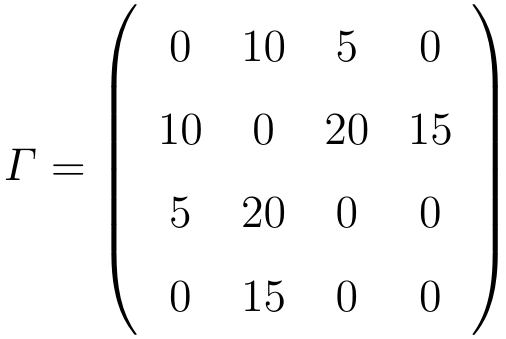
\includegraphics[width=0.3\textwidth]{adj_matrix3.png}}
	\hfil
	\subfigure[Κατευθυνόμενου γράφου $\hat{G_2}$]{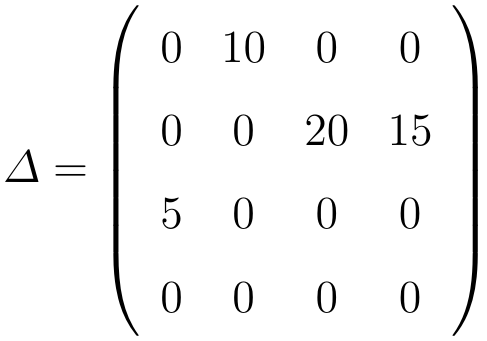
\includegraphics[width=0.3\textwidth]{adj_matrix4.png}}
\caption{Μητρώα γειτνίασης γράφων με βάρη}
 \label{mat2}
\end{figure*}

\setcounter{subfigure}{0}
\gr


\subsubsection{\gr Λίστες γειτνίασης}
\paragraph{}
Η λίστα γειτνίασης χρησιμοποιείται για την αναπαράσταση των κόμβων ενός γράφου, καθώς του συνόλου των γειτονικών τους κόμβων. Συγκεκριμένα, η λίστα γειτνίασης ενός πεπερασμένου γράφου $G=(V,E)$ είναι μία λίστα από $\abs{V}$ αταξινόμητες λίστες. Κάθε λίστα αντιστοιχεί και σε έναν κόμβο του γράφου, για τον οποίο η αντίστοιχη λίστα περιλαμβάνει το σύνολο των γειτονικών του κόμβων.  Στην περίπτωση βεβαρημένου γράφου, σε κάθε λίστα ενός κόμβου $V_i$ με $i=0,...,\abs{V}$, εκτός από την πληροφορία των γειτονικών κόμβων αποθηκεύονται επίσης και τα βάρη των αντίστοιχων ακμών μεταξύ του κόμβου $V_i$ και των γειτονικών του κόμβων. Για παράδειγμα, στα Σχήματα \ref{list1} και \ref{list2} παρουσιάζονται οι λίστες γειτνίασης των γραφών που μελετήθηκαν ως τώρα, των Σχημάτων \ref{gr} και \ref{gr2} αντίστοιχα. 

\gr
\begin{figure*}[h]
\centering
\subfigure[Μη κατευθυνόμενος γράφος]{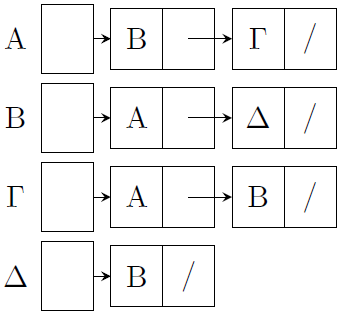
\includegraphics[width=0.34\textwidth]{adj_list1.png}}
	\hfil
	\subfigure[Κατευθυνόμενος γράφος]{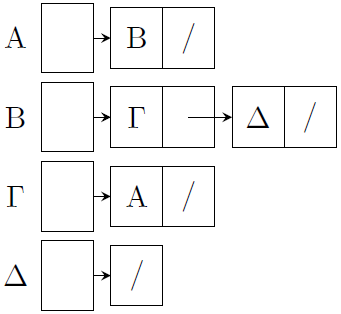
\includegraphics[width=0.34\textwidth]{adj_list2.png}}
\caption{Λίστες γειτνίασης γράφων χωρίς βάρη}
\label{list1}
\end{figure*}

\begin{figure*}[!ht]
\centering
\subfigure[Μη κατευθυνόμενος γράφος]{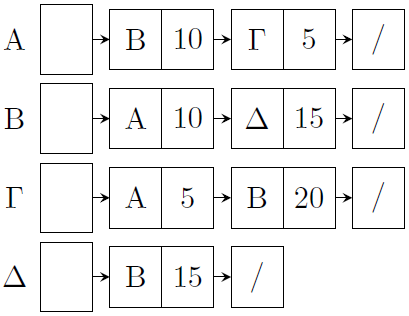
\includegraphics[width=0.4\textwidth]{adj_list3.png}}
	\hfil
	\subfigure[Κατευθυνόμενος γράφος]{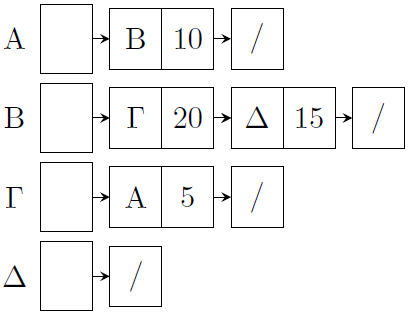
\includegraphics[width=0.4\textwidth]{adj_list4.png}}
\caption{Λίστες γειτνίασης γράφων με βάρη}
\label{list2}
\end{figure*}

Για την περαιτέρω κατανόηση των διαφορών μεταξύ των μητρώων και των λιστών γειτνίασης παρατίθεται ο Πίνακας \ref{adj}. Ο Πίνακας \ref{adj} παρουσιάζει συγκεντρωτικά τα κόστη της χρονικής πολυπλοκότητας εκτέλεσης διαφόρων βασικών ενεργειών, που εφαρμόζονται συχνά πάνω στους γράφους. Συγκεκριμένα, στη γενική περίπτωση οι λίστες γειτνίασης προτιμώνται για την αναπαράσταση αραιών γράφων. Ωστόσο στη χειρότερη περίπτωση όπου ο γράφος είναι πυκνός, τότε η πολυπλοκότητά τους ισούται με αυτή των μητρώων γειτνίασης. Το σημαντικότερο πλεονέκτημα των λιστών γειτνίασης είναι η άμεση προσπέλαση των γειτονικών κόμβων ενός δοθέντος κόμβου, σε σχέση με ένα μητρώο γειτνίασης. Η ιδιότητα αυτή των λιστών γειτνίασης είναι ιδιαίτερα σημαντική σε πρακτικές υλοποιήσεις πολλών αλγορίθμων. 


\gr
\begin{table}[ht]
\caption{\gr Χρονική πολυπλοκότητα ενεργειών πάνω στους γράφους}
\label{adj}
\centering
\begin{tabular}{| c | c | c |}
\hline
	 & \textbf{Λίστα Γειτνίασης} & \textbf{Μητρώο Γειτνίασης} \\
\hline
Αποθήκευση γράφου &  $O(\abs{V}+ \abs{E})$ & $O(\abs{V}^2)$  \\
\hline
Προσθήκη κόμβου & $O(1)$ & $O(\abs{V}^2)$ \\
\hline
 Προσθήκη ακμής &  $O(1)$ & $O(1)$  \\
\hline
 Αφαίρεση κόμβου & $O(\abs{E})$  &  $O(\abs{V}^2)$\\
\hline
 Αφαίρεση ακμής & $O(\abs{V})$ &  $O(1)$\\
\hline
 Έλεγχος γειτνίασης 2 κόμβων & $O(\abs{V})$ &   $O(1)$\\
\hline
\end{tabular}
\end{table}


\gr
\subsubsection{\gr Απλό διανυσματικό μοντέλο (\en VSM)}
\paragraph{}
Το διανυσματικό μοντέλο (\en Vector Space Model\gr) προέρχεται από το χώρο της ανάκτησης πληροφορίας, όπου είναι ιδιαίτερα διαδεδομένο \cite{baeza1999modern}. Η φιλοσοφία του μοντέλου βασίζεται στη δημιουργία ενός λεξικού, στο οποίο καταγράφεται για κάθε κείμενο το πλήθος εμφάνισης της κάθε λέξης.

Η λειτουργία του χαρακτηρίζεται από δύο στάδια. Αρχικά, προηγείται ένα στάδιο ευρετηρίασης όλων των κειμένων, όπου γίνεται καταγραφή όλων των λέξεων $w_i$, $i\in[1,M]$ που απαρτίζουν κάθε κείμενο, ενώ στη συνέχεια σε κάθε λέξη $w_i$ ενός κειμένου $d_j$, $j\in[1,N]$, ανατίθεται ένα βάρος \en TF-IDF (Term Frequency – Inverse Document Frequency) \gr σύμφωνα με τη Σχέση \ref{wei1}.

\begin{equation} \label{wei1}
    v_{i,j}=\left\{
                \begin{array}{ll}
                  (1+logf_{i,j})log\left(\frac{N}{n_i}\right),\; \alpha v \; f_{i,j}>0\\
                  0, \quad \alpha\lambda\lambda \iota\acute{\omega}s
                \end{array}
              \right.
\end{equation}
όπου:
\begin{description}

\item[f_{i,j}] είναι η συχνότητα της λέξης $w_i$ στο κείμενο $d_j$
\item[n_i] είναι το πλήθος των κειμένων στο οποίο εμφανίζεται η λέξη $w_i$
\item[N] είναι το συνολικό πλήθος των κειμένων
\end{description}

Τα βάρη \en TF-IDF \gr των λέξεων ενός κειμένου $d_j$ σχηματίζουν μια διανυσματική περιγραφή του κειμένου, ως $\vec{d_j}=(v_{1,j},v_{2,j},...,v_{M,j})$. Ενώ αντίστοιχα, τα βάρη \en TF-IDF \gr των λέξεων του κάθε κειμένου $d_j$, για $\forall j \in[1,N]$, σχηματίζουν ένα μητρώο βαρών $U_{i,j}$ διαστάσεων $M\times N$,  μεταξύ των λέξεων $w_i$ και των κειμένων $d_j$ ως εξής:

\[U_{i,j}=
  \left( {\begin{array}{cccc}
    v_{1,1}       & v_{1,2} & \dots & v_{1,M} \\
    v_{2,1}       & v_{2,2}  & \dots & v_{2,M}  \\
    \vdots & \vdots & \ddots  & \vdots \\
    v_{N,1}       & v_{N,2}  & \dots & v_{N,M} 
  \end{array} } \right)
\]




%ΑΝΑΛΥΣΗ ΧΡΟΝΟΣΕΙΡΩΝ
\newpage
\thispagestyle{plain}
\null
\vspace{2cm}
\hspace{-6.5mm}{\textbf{\Huge
 \gr Κεφάλαιο 3}}
\vspace{-4mm}
\section{\gr Ανάλυση Χρονοσειρών}
\lettrine[loversize=0.03]{\en M\gr}{\gr ια} 
χρονοσειρά είναι μία ακολουθία από καλά ορισμένα σημεία δεδομένων σε σταθερά χρονικά διαστήματα μίας χρονικής περιόδου. Η ανάλυση χρονοσειρών αναφέρεται στη χρήση στατιστικών μεθόδων για την μελέτη αυτών των χρονικών σημείων, με σκοπό την εξαγωγή χρήσιμων στατιστικών και χαρακτηριστικών των δεδομένων. Το μεγαλύτερο πλεονέκτημα της ανάλυσης των χρονοσειρών αποτελεί η δυνατότητα αξιοποίησής τους για την κατανόηση των ήδη υπαρχουσών δεδομένων, αλλά και για τη μελέτη των μελλοντικών τιμών.  



\subsection{\gr Βασικές έννοιες}
\paragraph{}
Επίσημος ορισμός μίας χρονοσειράς δεν υπάρχει, καθώς υπάρχει μία πληθώρα εναλλακτικών ορισμών. Πολλοί ορισμοί περιγράφουν μία χρονοσειρά ως μία ακολουθία αποκλειστικά αριθμητικών τιμών, ενώ άλλοι θεωρούν ότι οι τιμές αποτελούν σαφή ορισμένα και ισαπέχοντα χρονικά σημεία. Συνεπώς, για την περιγραφή ενός γενικού μοντέλου χρονοσειράς δίνονται οι Ορισμοί 1 και 2 \cite{dunham2003data}.\\

\hspace{-7.7mm}
\textbf{Ορισμός 1:} \textit{Δοθείσης μιας διάστασης δεδομένων, $D$ μια \textbf{χρονοσειρά} είναι ένα σύνολο από $n$ τιμές: $\{<t_1,d_1>,<t_2,d_2>,...,<t_n,d_n>\}$. Σε κάθε χρονική στιγμή $t_i$, όπου $i\in[1,n]$, αντιστοιχεί μία τιμή δεδομένων $d_i$. Στην περίπτωση όπου οι τιμές ορίζονται σε συγκεκριμένες και καλά ορισμένες χρονικές στιγμές, τότε οι τιμές αυτές μπορούν να αναπαρασταθούν σαν ένα διάνυσμα $<d_1,d_2,...,d_n>$.}\\


\textbf{Παράδειγμα παρουσιάσης αλγορίθμου:}\\

\hrule
\vspace{2mm}
\hspace{-7mm}
\textbf{Αλγόριθμος 1:} Κατασκευή του \en Twitter keepup \gr γράφου\\
\vspace{-6mm}
\hrule
\vspace{2mm}
\hspace{-8mm}
\textbf{Είσοδος:} Ένα σύνολο κόμβων \textit{\en N\gr}, ένα κατώφλι \textit{\en th\gr}, μία συνάρτηση για τον υπολογισμό
%\vspace{-1mm}
\null\hspace{10mm} της \textit{απόστασης}\\
\textbf{Έξοδος:} Ο \en keepup \gr γράφος \textit{\en $G_{th}$(N,E)} \gr \\
\vspace{-10mm}
\begin{itemize}
\item[1:] $E$ = κενό
\vspace{-4mm}\item[2:] \textbf{για κάθε}  $(n_i, n_j) \in N$ \textbf{κάνε} 
\vspace{-4mm}\item[3:] \hspace{8mm}$keepup(n_i,n_j)= 1-(|distance(N_c, N_i)-distance(N_c, N_j)|)$
\vspace{-4mm}\item[4:] \hspace{8mm}$e_{ij}=keepup(n_i,n_j$)
\vspace{-4mm}\item[5:] \hspace{8mm}\textbf{αν} $e_{ij}<= th$ \textbf{τότε}  
\vspace{-4mm}\item[6:] \hspace{8mm}\hspace{8mm}$E=E \cup e_{ij}$
\vspace{-4mm}\item[7:] \hspace{8mm}\textbf{τέλος αν}
\vspace{-4mm}\item[8:] \textbf{τέλος για}
\end{itemize}
\vspace{-2mm}
\hrule
\
\\


%\newpage
%\thispagestyle{empty}
%\null


\newpage
\gr
\en
\thispagestyle{plain}
\renewcommand{\bibname}{\gr Βιβλιογραφία}
\bibliographystyle{apa}%unsrt}
\bibliography{sample}
\end{document}